\subsection{Regular (Baryonic) Matter}

In our normal day to day life we meet protons, neutrons, and electrons. There are also other particles we come across, such as neutrinos, muons, taus, etc. Another particle we meet often is the photon, and some others we won't get into.

When the universe came into being in the big bang quarks and photons were created. those quarks then combined into protons and neutrons. protons are basically hydrogen nuclei, so hydrogen was created in the big bang. For a short period of time after the big bang there were conditions for nuclear fusion across the early universe, so about 10\% of the matter created from the big bang ended up being helium, and in terms of mass it was about 25\% (Because Helium is heavier than hydrogen). Elements heavier than helium weren't created at any significant quantities in the big bang. If we plot this on a graph:

% INSERT GRAPH

\begin{wrapfigure}[19]{r}{0pt}
	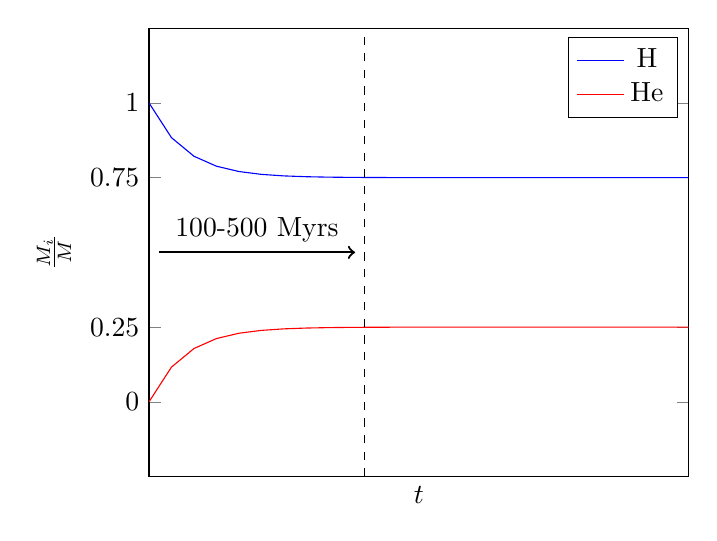
\begin{tikzpicture}
		\begin{axis}[xlabel=$t$, ylabel=$\frac{M_i}{M}$, ymin=-0.25, ymax=1.25, xmin=0, xmax=15, ytick={0,0.25,0.75,1}, yticklabels={0,0.25,0.75,1}, xtick=\empty]
			\addplot[domain=0:15, color=blue]{0.25*e^(-x)+0.75};\addlegendentry{H}
			\addplot[domain=0:15, color=red]{0.25 - 0.25*e^(-x)};\addlegendentry{He}
			\draw[dashed] (axis cs:6,-0.25) -- (axis cs:6,1.25);
			\node (n1) at (axis cs:0,0.5) {};
			\node (n2) at (axis cs:6,0.5) {};
			\draw[->, thick] (n1) -- (n2) node [above, pos=0.5]{100-500 Myrs};
		\end{axis}
	\end{tikzpicture}
	\caption{The portion of mass of the universe by element in the universe's early times.}
\end{wrapfigure}


The portion of mass of hydrogen of the total mass is denoted by $X$, hydrogen by $Y$, and metals, which are all the elements heavier than helium and are denoted by $Z=\frac{M_{metals}}{M}$. For our sun:

\begin{align}
	X_\mathSun &= 0.7381\\
	Y_\mathSun &= 0.2485\\
	Z_\mathSun &= 0.0134
\end{align}

The above was a discussion for gas and plasma. There is another kind of matter in space called dust. Dust is similar to the dust we know. It's particles about a micrometer in diameter made of water, carbon, silica, etc. Why do we mention this? In terms of the mass of the metals in the universe, about half of it is dust. Moreover, dust is a significant factor in observations of the universe, either in interfering in our ability to see things or in creating conditions that allow us to infer information. Dust also aids the creation of molecules by speeding up processes which are very slow in gasses.

An important definition for us will be the "average mass" which we'll use in many formulas. Assume we have a box filled with hydrogen and some helium and some metals, all with the relative quantities that are in the sun. What would the average mass per particle be? approximately a proton mass. And if the gas in the box is ionized? 0.5 proton masses. This is because we doubled the number of particles by freeing the electrons, which have approximately 0 mass relatively to the protons. This was a back of the napkin approximation just for sanity check and to have an idea of what we're expecting. The exact calculations is:

\begin{align}
	\overline{m} = \frac{\sum\limits_j N_jm_j}{\sum\limits_j N_j}
\end{align}

where $j$ is each element type, N is their number, and m their mass. Rewriting in terms of $X$,$Y$,$Z$:

\begin{align}
	\frac{1}{\overline{m}} &= \frac{\sum N_jM_j}{\sum N_jm_jM_j}\\
	&= \frac{M_j}{M_{tot}}\cdot\sum\frac{N_j}{M_j}\\
	&= \frac{1}{m_H}\ins{X+\frac{1}{4}Y + \frac{1}{A_Z}Z}
\end{align}

% FIX MISTAKE FROM RESHIMOT

where

\begin{equation}
	M_j = \begin{cases}
		N_Hm_H & H\\
		N_{He} \cdot 4m_H & He\\
		N_ZA_Z & else
	\end{cases}
\end{equation}

Sometimes the following definition is used:

\begin{equation}
	\mu = \frac{\overline{m}}{m_H}
\end{equation}

and if we plug in the numbers for the sun we indeed find that it's very close to 1. We won't do this explicitly because there's a correction for the formula for a non-neutral gas, which our sun is not. For a completely ionized gas, i.e all the electrons are free, we just need to change $N_j$:

\begin{equation}
	N_j = \begin{cases}
		1\rightarrow2 & H\\
		1\rightarrow3 & He\\
		1\rightarrow\left\langle\frac{A_Z}{2}\right\rangle & Else
	\end{cases}
\end{equation}

Which gives us, for a completely ionized gas:

\begin{equation}
	\mu = \left[2X+\frac{3}{4}Y+\frac{1}{2}Z\right]^{-1}
\end{equation}

and if you insert the numbers for our sun we find

\begin{align}
	\left\langle A\right\rangle &= 15-16\\
	\mu_\mathSun &\simeq 0.6
\end{align}
